\section{Introduction}
    Melanoma is a type of skin cancer, develops in the cells (melanocytes) that produce melanin — the pigment that gives your skin its color, The exact cause of all melanomas isn't clear, but exposure to ultraviolet (UV) radiation from sunlight increases your risk of developing melanoma. ~\cite{mayo2022}

    melanoma is more dangerous because of its ability to spread to other organs more rapidly if it is not treated at an early stage. ~\cite{scfm2022}

    At present, CNN has achieved very good performance in the field of computer vision, such as object detection, image recognition, classification, etc. 

    Convolutional Neural Network (CNN) is a type of deep learning model for processing data that has a grid pattern, such as images, which is designed to automatically and adaptively learn spatial hierarchies of features. CNN is a mathematical construct that is typically composed of three types of layers (or building blocks): convolution, pooling, and fully connected layers. The first two, convolution and pooling layers, perform feature extraction, whereas the third, a fully connected layer, maps the extracted features into final output, such as classification. A convolution layer plays a key role in CNN, which is composed of a stack of mathematical operations, such as convolution, a specialized type of linear operation. \cite{Yamashita2018}

    Because of the difficulty of detecting melanoma cancer in an ordinary way CNN is used to classify melanoma skin cancer.

    Research on the classification and detection of melanoma cancer by various methods has been carried out. In 2016 there was a paper entitled "Deep Residual Learning for Image Recognition" using the ResNet architecture. The paper was a winner at the 2015 ILSVRC (Imagenet competition). ~\cite{Arief2019}


\section{Proposed Convolutional Neural Network Model}
    The main aim of this implementation is to detect melanoma skin cancer through RGB images, to achieve this, we build a deep learning model that is capable of extracting features from the given dataset.

    After delving into many articles and studies, we have found that the best convolutional neura network model we can suggest in this case is resnet50 and so we are going to implement i from scratch. as shown in figure ~\ref{fig:architecture}

    \begin{figure}[htbp]
    \begin{center}
    
\includegraphics[width=15cm]{./chapter-05-our-contribution/3.png}
    \end{center}
    \caption{proposed architecture which we have used for melanoma recognition}
    \label{fig:architecture}
    \end{figure}

\section{Dataset (MNIST- HAM10000)}

    The ISIC archive is the largest public database for dermatoscopic image analysis research, and where the original HAM10000 was made available.~\cite{JULIANA2021}

    The HAM10000 dataset is composed of 10.015 dermatoscopic images of pigmented skin lesions. The data was collected from Australian and Austrian patients. Two institutions participated in providing the images: Cliff Rosendahl in Queensland, Australia, and Medical University of Vienna, Austria. According to the authors, seven classes are defined on this dataset where some diagnoses were unified into one class for simplicity. Information regarding patient age, sex, lesion location and diagnosis is also provided with each image. ~\cite{JULIANA2021}


    The dataset has been collated and published by Tschandl, P., Rosendahl, C. \& Kittler, H.~\cite{JULIANA2021} A sample of each type of skin lesion present in the dataset is demonstrated in the figure ~\ref{fig:dataset}. and the distribution of lesions is show in figure ~\ref{fig:distribution}

    \begin{figure}[htbp]
    \begin{center}
    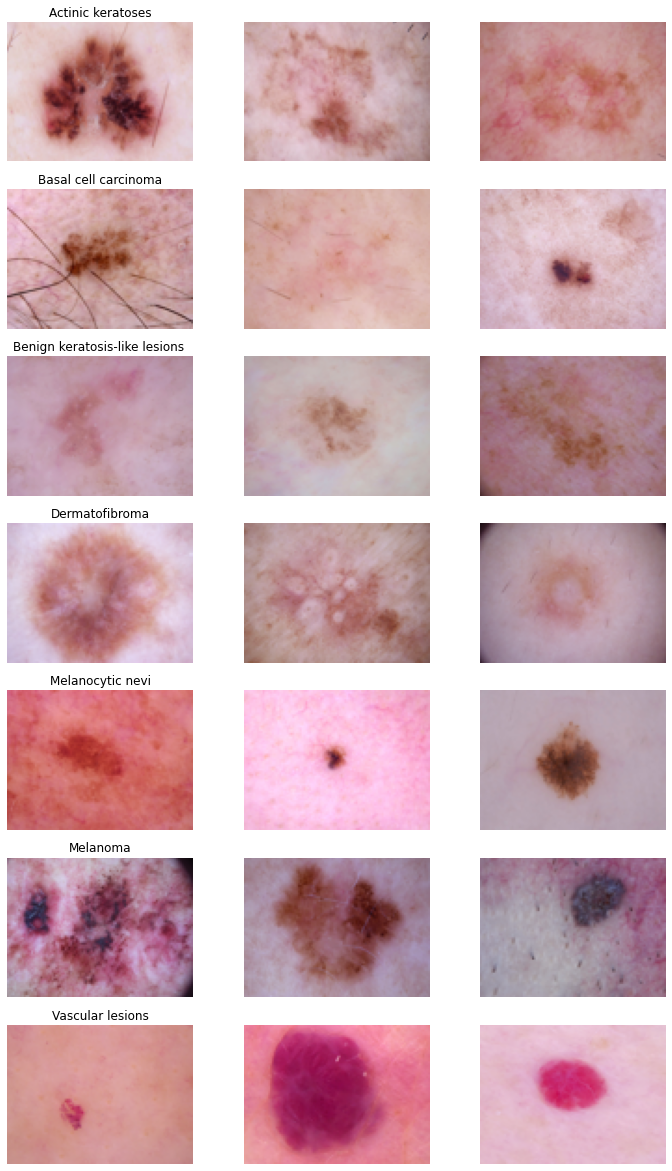
\includegraphics[width=12cm]{./chapter-05-our-contribution/2.png}
    \end{center}
    \caption{A sample of each type of skin lesion ~\cite{JULIANA2021}}
    \label{fig:dataset}
    \end{figure}

    

    \begin{figure}[htbp]
    \begin{center}
    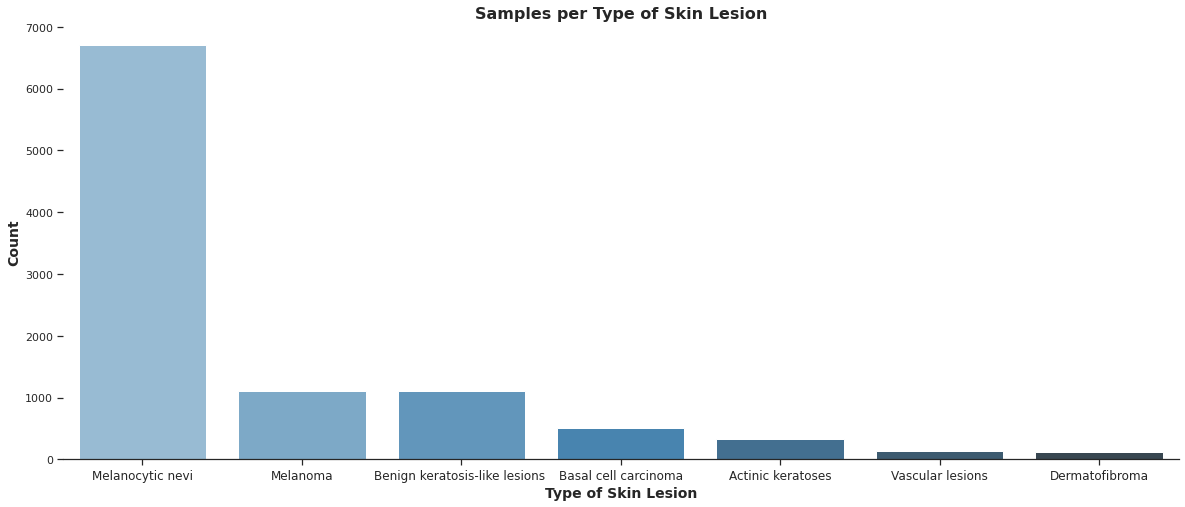
\includegraphics[width=15cm]{./chapter-05-our-contribution/5.png}
    \end{center}
    \caption{This count plot helps to understand the distribution of the data. ~\cite{JULIANA2021}}
    \label{fig:distribution}
    \end{figure}

\section{Pre-processing}
    Before starting the model training process we need to process the dataset, as we learned earlier the dataset consists of around 10015 labeled images for 7 different types of skin lesions, but in our case, we want to get images classified on only two types of skin lesions (Melanoma and Not melanoma). We do this in several steps:

    \begin{description}
        \item[Data cleansing: ] \hfill \\  In this step, we remove unused and damaged data, also repair data that is incorrectly formatted.

        \item[Data separation: ] \hfill \\  After cleansing the data set, we separate the data set into two types of skin lesions by changing the data label for the non-melanoma types to non-melanoma and we keep the data label for the type of melanoma as it is.

        \item[Data balancing: ] \hfill \\  When reclassifying the data set, we notice that the data set is numerically unbalanced. To solve this problem, we increase the number of images of the melanoma type by rotating, cropping and scaling. As for the non-melanoma type, we reduce the number of images by randomly selecting a specified number of images.

        \item[Image resizing: ] \hfill \\  In this step, we reduce the image size to 75*100 to speed up the training process of the deep learning model. data splitting : Before the data set becomes usable, we divide it into two parts, the first part is the training set with 80 percent, and the second part is the test set with 20 percent
    \end{description}

        The diagram ~\ref{fig:steps} helps to understand these steps

        \begin{figure}[htbp]
        \begin{center}
        
\includegraphics[width=15cm]{./chapter-05-our-contribution/4.png}
        \end{center}
        \caption{Pre-processing}
        \label{fig:steps}
        \end{figure}



\section{Experimental results}
    To judge the performance of the model for the task of predicting skin lesions, we use several evaluation metrics to evaluate our model. This is because the model may perform well using one measurement from one evaluation metric, but may perform poorly using another measurement from another evaluation metric. Using evaluation metrics are critical in ensuring that our model is operating correctly and optimally.

    When the model was trained for 30 epochs, it was observed that the accuracy for both the training and test data started with rather large values and continued to increase small from epoch 4 until it reached its peak in epoch 30, where the test accuracy reached 93 percent and the training accuracy was 97 percent.

    The plot for the accuracy and loss obtained during the training and testing process is shown in Figure ~\ref{fig:acc-loss}

    \begin{figure}[htbp]
    \begin{center}
    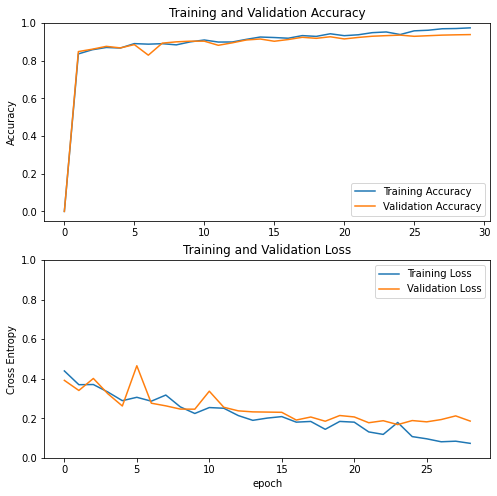
\includegraphics[width=15cm]{./chapter-05-our-contribution/1.png}
    \end{center}
    \caption{Accuracy and Loss}
    \label{fig:acc-loss}
    \end{figure}

    The table ~\ref{tab:eval} also includes several other measurements that we used in evaluating our model

    \setlength{\arrayrulewidth}{0.5mm}
    \setlength{\tabcolsep}{18pt}
    \renewcommand{\arraystretch}{1.5}

    \begin{table}[htbp]
    \begin{center}
        \begin{tabular}{|c|c|c|c|c|}
        \hline 
        Classes & Precision & Recall & F1-score & Support \\ 
        \hline 
        Non-melanoma & 0.95 & 0.93 & 0.94 & 1293 \\ 
        \hline 
        Melanoma & 0.93 & 0.95 & 0.94 & 1226 \\ 
        \hline 
        \end{tabular} 
    \end{center}
    \caption{Evaluation Mesures}
    \label{tab:eval}
    \end{table}






